\documentclass[noamssymb,svgnames]{beamer}
\usecolortheme{beaver}
\useinnertheme[shadow]{rounded}
\usefonttheme{serif}
\usefonttheme{professionalfonts}

\usepackage[bitstream-charter]{mathdesign} % Use BT Charter font
\usepackage[T1]{fontenc}                   % Use T1 encoding instead of OT1
\usepackage[utf8]{inputenc}                % Use UTF8 input encoding
\usepackage{microtype}                     % Improve typography
\usepackage{booktabs}
\usepackage[binary-units]{siunitx}
\usepackage{tikz}
\usetikzlibrary{shapes.geometric,arrows}

\usepackage[vlined]{algorithm2e}

\usepackage{hyperref}
\hypersetup{pdfstartview=Fit}

% BEAMER CONFIGURATION ---------------------------------------------------------
\setbeamerfont{block title}{size=\normalsize}
\setbeamerfont{block body}{size=\scriptsize}
\setbeamercolor{block title}{fg=darkred,bg=gray!10!white}
\setbeamercolor*{item}{fg=darkred}

% MINTED CONFIGURATION ---------------------------------------------------------
\usepackage[many,minted]{tcolorbox}

% Set ipython options
\setminted{
  mathescape,
  autogobble,
  fontfamily=courier,
  framesep=2mm
}

% TIKZ CONFIGURATION -----------------------------------------------------------
\tikzstyle{start} = [rectangle, draw, fill=green!20, rounded corners=3mm,
  centered, minimum height=1em]
\tikzstyle{end} = [rectangle, draw, fill=red!20, rounded corners=3mm,
  centered, minimum height=1em]
\tikzstyle{process} = [rectangle, draw, fill=yellow!20, text width=8em, text
  centered, minimum height=1em]
\tikzstyle{decision} = [diamond, draw, fill=gray!20, text width=5em, text badly centered,
  inner sep=0pt]
\tikzstyle{line} = [draw, -latex', thick]


\newcommand{\highlight}[1]{%
  \colorbox{yellow!20}{$\displaystyle#1$}}

% ------------------------------------------------------------------------------
\title{Monte Carlo for Particle Transport}

\institute{\includegraphics[width=2in]{../images/openmc_logo.png}}

\date{OpenMC Workshop \\ Canadian Nuclear Laboratories \\ March 14--16, 2017}

% ------------------------------------------------------------------------------
\begin{document}

\frame{\titlepage}

% ------------------------------------------------------------------------------
\begin{frame}{Monte Carlo method}
  \begin{itemize}
  \item Nuclear reactor analysis relies on ability to solve neutral particle
    transport
    \begin{itemize}
    \item \emph{Deterministic methods:} discrete ordinates, method of
      characteristics, collision probability method, diffusion theory
    \item \emph{Monte Carlo method:} directly simulate life of individual
      particles (neutrons, photons) using known probability distributions
    \end{itemize}
  \item MC method confers a number of benefits:
    \begin{itemize}
    \item Use of continuous-energy interaction data (no grouping necessary)
    \item No spatial approximations necessary
    \item Parallelization is ``simple'' since particles do not interact with one
      another
    \end{itemize}
  \item Biggest impediment to wider use is \emph{time to solution}
  \end{itemize}
\end{frame}

\begin{frame}{Adoption of MC}
  \begin{itemize}
  \item As computers continually improve in performance over time, the scope of
    problems amenable to solution by MC has increased as well
  \item Research, test, small reactors
  \item Lots of activity in the research community on MC methods, and plenty of
    new codes:
    \begin{itemize}
    \item \textbf{U.S.}: MC21, Shift, Mercury, OpenMC
    \item \textbf{China}: RMC, SuperMC
    \item \textbf{Europe}: Serpent
    \end{itemize}
  \end{itemize}
\end{frame}

\begin{frame}
  \centering
  \includegraphics[width=0.8\textwidth]{../images/standards.png}
\end{frame}

\begin{frame}{Neutral particle transport}
  \centering
  \resizebox{\textwidth}{!}{%
  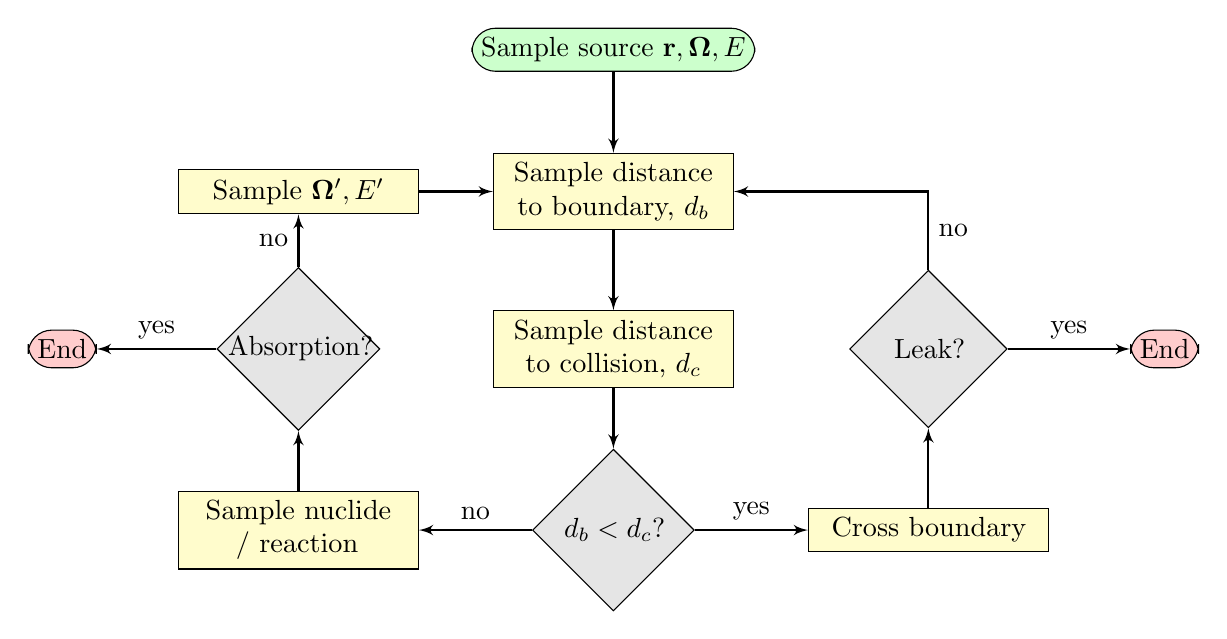
\begin{tikzpicture}[node distance=2cm]
    \node[start] (source) {Sample source $\mathbf{r}, \mathbf{\Omega}, E$};
    \node[process, below of=source, node distance=1.8cm] (db) {Sample distance to boundary, $d_b$};
    \node[process, below of=db] (dc) {Sample distance to collision, $d_c$};
    \node[decision, below of=dc, node distance=2.3cm] (dbdc) {$d_b < d_c$?};

    \node[process, right of=dbdc, node distance=4cm] (boundary) {Cross boundary};
    \node[decision, above of=boundary, node distance=2.3cm] (leak) {Leak?};
    \node[end, right of=leak, node distance=3cm] (leaked) {End};

    \node[process, left of=dbdc, node distance=4cm] (collision) {Sample nuclide / reaction};
    \node[decision, above of=collision, node distance=2.3cm] (absorb) {Absorption?};
    \node[end, left of=absorb, node distance=3cm] (dead) {End};
    \node[process, above of=absorb] (secondary) {Sample $\mathbf{\Omega'}, E'$};

    \path[line] (source) -- (db);
    \path[line] (db) -- (dc);
    \path[line] (dc) -- (dbdc);
    \path[line] (dbdc) -- node[above] {yes} (boundary);
    \path[line] (dbdc) -- node[above] {no} (collision);
    \path[line] (collision) -- (absorb);
    \path[line] (absorb) -- node[left] {no} (secondary);
    \path[line] (absorb) -- node[above] {yes} (dead);
    \path[line] (secondary) -- (db);
    \path[line] (boundary) -- (leak);
    \path[line] (leak) |- node[near start,right] {no} (db);
    \path[line] (leak) -- node[above] {yes} (leaked);
  \end{tikzpicture}
  }
\end{frame}

\begin{frame}{Tallies}
  Monte Carlo is well-suited to calculating volume integral quantities of the
  form:
  \begin{equation*}
    X = \int d\mathbf{r} \int d\mathbf{\Omega} \int dE \;
    f(\mathbf{r},\mathbf{\Omega},E) \psi (\mathbf{r},\mathbf{\Omega},E)
  \end{equation*}
  During a simulation, physical quantities of interest (called \emph{tallies}
  or \emph{detectors}) are accumulated as:
  \begin{equation*}
    \hat{X} = \frac{1}{N} \sum\limits_{i \in T} w_i \ell_i f_i
  \end{equation*}
\end{frame}

\begin{frame}{Statistics}
  At the end of a simulation, we have a set of realizations for each tally,
  $\hat{X}_1, \hat{X}_2, \dots, \hat{X}_N$. We can calculate mean and variance
  as
  \begin{align*}
    \bar{X} &= \frac{1}{N} \highlight{\sum\limits_{i=1}^N \hat{X}_i} \\
    s^2_X &= \frac{1}{N-1} \left ( \frac{1}{N} \highlight{\sum\limits_{i=1}^N \hat{X}_i^2} -
    \bar{X}^2 \right )
  \end{align*}
\end{frame}

\begin{frame}{Problem Types}
  \begin{itemize}
  \item For \textbf{fixed source} problems, the source of particles is known
    \emph{a priori}, e.g., 100 neutrons/sec from an isotropic point source
  \item When neutrons from fission are the primary source, the distribution of
    source sites is not known \emph{a priori} because it depends on the flux,
    which is what we're solving for
  \end{itemize}
\end{frame}

\begin{frame}{$k$ Eigenvalue Algorithm}
  \begin{algorithm}[H]
    \DontPrintSemicolon
    Guess initial source distribution and $k$\;
    \For {$i = 1 \to n_{generations}$}{
      \For {$j =1 \to n_{particles}$}{
        Sample neutron from source bank\;
        Track neutron until death, at each {\bf collision} storing
        \begin{equation*}
          n = \left \lfloor \frac{\nu\Sigma_f}{\Sigma_t} + \xi \right
          \rfloor \quad \text{fission sites}
        \end{equation*}\;
      }
      Sample $N = n_{particles}$ neutrons from $N'$ fission sites collected\;
      Calculate $k^{(i)} = N'/N$\;
    }
  \end{algorithm}
\end{frame}

\begin{frame}{Inactive generations}
  \begin{itemize}
  \item Our goal is to estimate physical quantities (e.g. $^{235}$U fission
    rate) resulting from a source
  \item In the generation algorithm, we have to wait until the spatial
    distribution of source sites converges (otherwise, our results would be
    biased by the arbitrary source guess)
  \item Simulation is broken up into \emph{inactive} and \emph{active}
    generations
  \item For problems with large dominance ratio, hundreds of generations may
    need to be discarded
  \end{itemize}
\end{frame}

\end{document}
